\documentclass[conference]{IEEEtran}
\usepackage{cite}
\usepackage{amsmath,amssymb}
\usepackage{graphicx}
\usepackage[hidelinks]{hyperref}
\graphicspath{{assets/}}
\newcommand{\CleanWins}{1}
\newcommand{\AblationWins}{3}
\newcommand{\NoisyWins}{4}
\newcommand{\BestReduction}{0.71}
\newcommand{\GammaZeroMin}{43}
\newcommand{\GammaZeroMax}{57}


\title{Measurement-Aware Regularization in Finite-Shot Quantum Feature Regression}
\author{\IEEEauthorblockN{Kartik Mehra}
\IEEEauthorblockA{Team Outliers\\kartik.mehra2024@nst.rishihood.edu.in}
\and
\IEEEauthorblockN{Viraj Chafale}
\IEEEauthorblockA{Team Outliers\\viraj.chafale2024@nst.rishihood.edu.in}}

\begin{document}
\maketitle

\begin{abstract}
Quantum features estimated using finite measurement shots contain sampling uncertainty even without device errors. This semester project implements a fixed two-qubit feature map and investigates whether classical readout regularization improves prediction under limited measurements. An initial ordinary least squares and Ridge comparison is extended with diagonal and full within-setting covariance penalties estimated from training measurements. The extension evaluates two synthetic targets at 32, 128 and 512 shots per setting on twenty fresh datasets, with five acquisitions per dataset and 32 validation candidates per regularized method. Full covariance regularization improves the primary clean-label mean error relative to Ridge in only \CleanWins{} of six finite-shot settings, by approximately \BestReduction{}\% in that setting. The off-diagonal ablation and a separate noisy-label analysis also give mixed outcomes. Independent numerical audits and 54 automated tests verify the implementation and saved results. The contribution is a reproducible adaptation and controlled evaluation of established methods, including negative findings; no new algorithm, general superiority or quantum advantage is claimed.
\end{abstract}

\begin{IEEEkeywords}
quantum machine learning, finite-shot measurements, quantum features, Ridge regression, covariance regularization
\end{IEEEkeywords}

\section{Introduction}
Quantum machine learning can use quantum circuits to transform classical inputs into measured features, followed by a classical predictor. In regression, expectation-value estimates become numerical inputs to a readout that predicts a continuous target. A finite number of circuit executions, or shots, produces sampling uncertainty even if the quantum circuit is ideal. Prior research studies finite-sampling noise, its effect on learning and strategies for reducing its influence~\cite{kreplin,hu2023}.

Additional shots generally improve individual feature estimates but consume more measurement resources. Predictive performance also depends on the target, representation, available data and estimator. Consequently, the most precise measurements do not by themselves establish the best allocation of learning resources, and a regularizer need not improve every task.

Ridge regression shrinks coefficient magnitude. Measurement-aware regularization instead can also penalize feature combinations according to their estimated sampling uncertainty. A covariance penalty distinguishes fluctuations shared by features extracted from the same shot. Such readout penalties already exist in the literature~\cite{baumann}; this project implements an adaptation rather than proposing a new principle.

The project addresses a semester-scale question: does this additional information improve regression compared with a well-tuned Ridge baseline under matched measurement budgets? A diagonal ablation tests whether off-diagonal covariance adds value. The resulting contribution consists of a verified circuit and covariance implementation, a paired fresh-seed evaluation, preserved raw measurements and an explicit analysis of failure cases. The quantum gates remain fixed throughout; only classical readout parameters are trained.

\section{Literature Review}
Kreplin and Roth~\cite{kreplin} introduce variance regularization for trainable quantum neural networks. Their investigated models reduce measured output noise by explicitly including variance in training. Our coefficient and covariance penalties operate on a fixed feature map and do not reproduce their trainable-circuit procedure or reported reduction factors.

Hu et al.~\cite{hu2023} characterize the learning capacity of sampled physical systems and introduce eigentasks that distinguish feature combinations by signal and noise properties. Hu and Gao~\cite{hu2024} analyse finite datasets together with finite measurement shots. These studies motivate noise-aware representations and careful generalization analysis. Eigentask learning and their analytical formulas are not implemented or validated here.

Lo Monaco et al.~\cite{shots} identify a finite-shot instability in a quantum linear-regression setting where sampling populates directions absent from ideal feature vectors. Their subsequent preprint~\cite{triple} incorporates explicit Ridge regularization when analysing prediction-error structure. Our local-observable features, fixed dimensionality and sample count are different. The experiment does not demonstrate their noise-only direction mechanism or a triple-descent law.

Baumann et al.~\cite{baumann} examine alternative organizations of a shared measurement record and describe covariance-regularized expectation-value training, Cov-EV, as a control. Their analysis relates grouped linear-readout training to a quadratic covariance penalty. This is the closest methodological precedent for the extension. We use a two-qubit static regression setup rather than their forecasting pipeline, so numerical errors cannot be compared directly.

The software implementation uses scikit-learn Ridge~\cite{sklearn} and an independent PennyLane circuit check~\cite{pennylane}. The literature review is targeted rather than exhaustive. The arXiv-only works are cited as preprints, not as accepted conference publications.

\section{Problem Statement and Objectives}
The input to a classical readout is a finite-shot estimate, not the ideal quantum feature vector. Sampling fluctuations can alter the fitted coefficients and subsequent predictions. Uniform coefficient shrinkage may not account for unequal and correlated measurement fluctuations. However, estimating a more structured penalty introduces its own uncertainty and selection choices.

The problem is to determine whether measurement-aware regularization improves held-out regression accuracy in a controlled small quantum-feature model. The primary comparison is FullCov versus Ridge on clean-label finite-shot test MSE. The ablation compares FullCov with DiagonalCov. A separate noisy-label condition probes sensitivity to imperfect supervised targets.

The objectives are to implement joint-outcome feature sampling, estimate measurement covariance from training records, train four readouts using a predefined selection procedure, and verify the resulting coefficients, predictions and statistics independently. Improvement is an empirical hypothesis, not an assumed outcome.

\section{Methodology}
\subsection{Circuit and Feature Construction}
The circuit starts in $|00\rangle$. In order, it applies $R_y(x)$ and $R_z(0.4x)$ to qubit 0; $R_y(2x+0.3)$ and $R_z(-0.7x)$ to qubit 1; CNOT$(0,1)$; $R_y(0.7)$ to qubit 0; $R_y(-0.4)$ and $R_z(0.2)$ to qubit 1; and CZ$(0,1)$. These constants are not optimized or selected using test error (Fig.~\ref{fig:circuit}).

Three independent settings measure both qubits in X, Y and Z. Each returns two single-qubit estimates and their pair product, giving
\begin{equation}
\begin{split}
\boldsymbol\phi(x)=(&\langle X_0\rangle,\langle X_1\rangle,\langle X_0X_1\rangle,
\langle Y_0\rangle,\langle Y_1\rangle,\\
&\langle Y_0Y_1\rangle,\langle Z_0\rangle,\langle Z_1\rangle,\langle Z_0Z_1\rangle).
\end{split}
\end{equation}
X measurement uses H before computational-basis measurement; Y uses $S^\dagger$ followed by H. Z needs no rotation. S shots per setting therefore cost 3S executions per input.

\begin{figure*}[t]
\centering
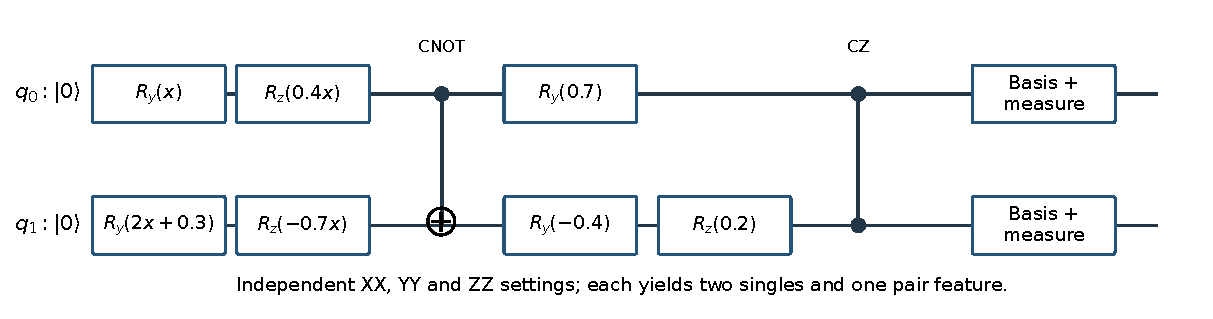
\includegraphics[width=0.96\textwidth]{circuit.pdf}
\caption{Fixed two-qubit feature map. Independent XX, YY and ZZ settings each yield two single-qubit estimates and one pair estimate. Only the classical readout is trained.}
\label{fig:circuit}
\end{figure*}

Born probabilities are calculated from an explicit NumPy statevector. Multinomial sampling draws joint outcome counts rather than adding arbitrary Gaussian errors to features. A shared shot supplies $v=(z_0,z_1,z_0z_1)^T$, with $z_j\in\{-1,+1\}$. This preserves within-setting sampling correlations. For an individual observable with mean $f(x)$, independent shots give $\operatorname{Var}(\widehat f_S\mid x)=(1-f(x)^2)/S$. This feature-precision relation is not a prediction-error guarantee.

\subsection{Training-Only Measurement Covariance}
For a fixed input and setting, let $m=S^{-1}\sum_s v_s$. The unbiased sample covariance of the estimated mean is
\begin{equation}
\widehat C_{i,g}=\frac{\sum_s v_sv_s^T-Smm^T}{S(S-1)}.
\label{eq:covariance}
\end{equation}
The four joint counts suffice to reconstruct the sums in (\ref{eq:covariance}); additional shots are unnecessary. This covariance measures uncertainty at a fixed input, not variation of features across different inputs.

Independent setting acquisitions give a block-diagonal $9\times9$ noise matrix. Average these matrices over training inputs only. If training-only standardization uses diagonal scale matrix D, propagate uncertainty as $\widehat C_z=D^{-1}\overline C D^{-1}$. FullCov retains the three within-setting blocks; DiagonalCov removes their off-diagonal terms. Numerical eigenvalues below zero but above $-10^{-12}$ are clipped to zero; more negative values are treated as an implementation error.

\subsection{Readout Models}
For standardized features z, predictions are
\begin{equation}
\widehat y=b+w^Tz.
\end{equation}
OLS minimizes training MSE. Ridge adds $\lambda\|w\|_2^2$. Both covariance models minimize
\begin{equation}
\begin{aligned}
L(b,w)={}&\frac1{n_{\rm tr}}\sum_i(y_i-b-w^Tz_i)^2\\
&+\lambda\|w\|_2^2+\gamma w^T\widehat C_z w,
\end{aligned}
\label{eq:loss}
\end{equation}
using either the diagonal or full within-setting covariance. The intercept is unpenalized. The implementation centers the training variables and solves the resulting regularized linear system. This is an empirical penalty, not an unbiased feature-noise correction. Setting $\gamma=0$ recovers Ridge at the same $\lambda$.

\begin{figure}[t]
\centering\small
\begin{tabular}{c}
\fbox{\parbox{0.85\columnwidth}{\centering Generate inputs, targets and fixed splits}}\\[3pt]
$\downarrow$\\[3pt]
\fbox{\parbox{0.85\columnwidth}{\centering Fixed circuit and joint XX/YY/ZZ measurements}}\\[3pt]
$\downarrow$\\[3pt]
\fbox{\parbox{0.85\columnwidth}{\centering Training-only scaling and covariance estimation}}\\[3pt]
$\downarrow$\\[3pt]
\fbox{\parbox{0.85\columnwidth}{\centering Fit candidates; select penalties on validation data}}\\[3pt]
$\downarrow$\\[3pt]
\fbox{\parbox{0.85\columnwidth}{\centering Held-out predictions, paired summaries and audit}}
\end{tabular}
\caption{Evaluation workflow. Both baselines and covariance methods share the same measurements. Test targets do not select parameters.}
\label{fig:workflow}
\end{figure}

\section{Experimental Design}
\subsection{Original Baseline and Fresh Extension}
The preserved initial study compares OLS and Ridge on five datasets. Its 600 finite-shot and 40 exact-feature evaluations use eight Ridge candidates. Its results motivated an extension, but they are not pooled with the new study.

The extension protocol was recorded before evaluating fresh dataset seeds 1001--1020 and acquisition seeds 2101--2105. These are disjoint from the original seeds. No method or penalty was selected using the new test results. Both phases use $x\sim\mathcal U[-\pi,\pi]$, with targets
\begin{equation}
f_1(x)=\sin x,\qquad f_2(x)=\sin(2x)+0.3\cos(3x).
\end{equation}
Each dataset has 64 training, 32 validation and 128 test inputs. The primary condition has clean labels. A separately reported sensitivity condition adds independent Gaussian noise of SD 0.1 to training and validation labels. Test error always uses the known noiseless target. It therefore measures latent-function estimation, not prediction of noisy observed test labels.

Shots per setting are 32, 128 and 512. Training, validation and test use the same budget within a condition and separate acquisitions. Exact simulator features provide diagnostic references with zero measurement covariance. They are not a free physical measurement method.

\subsection{Selection and Fairness}
StandardScaler is fitted only to training features. Covariance uses only training counts. Ridge searches 32 unique lambdas: 26 logarithmically spaced values from $10^{-6}$ to 10 plus the original eight values, removing duplicate endpoints. Thus it includes every Ridge-only option available to the new methods.

Each covariance method searches the original eight lambdas crossed with $\gamma\in\{0,0.1,1,10\}$, also 32 candidates. Minimum validation MSE selects the fit. Ties prefer smaller gamma, then smaller lambda; Ridge ties prefer smaller lambda. There is no train-plus-validation refit. Scikit-learn's summed-loss convention uses $\alpha=n_{\rm tr}\lambda$.

Equal candidate counts control one source of computational imbalance, but do not make the model families equally complex. The covariance grids have a coarser lambda resolution and an extra selection dimension. Both covariance models share identical grids, making the diagonal/full ablation particularly informative. At zero covariance their selected fits can differ from the finer Ridge grid for selection reasons unrelated to measurement covariance.

\subsection{Outcomes and Uncertainty}
The primary metric is held-out MSE. Coefficient norms, selected penalties and gamma-zero frequencies are diagnostics. Five acquisitions are averaged within each dataset before calculating the mean and sample SD across twenty dataset means. For paired contrasts, the reference-minus-candidate error difference is formed on shared records and similarly aggregated. Positive differences favour the candidate. SDs describe dispersion; they are not confidence intervals, and no statistical-significance claim is made.

The extension records 4,800 finite-shot and 320 exact-reference readouts. Internal tuning involves 124,160 candidate fits, including OLS. These are not independent datasets. The 300 unique acquisitions cost
\begin{equation}
B=20\cdot5\cdot224\cdot3\cdot(32+128+512)=45{,}158{,}400
\end{equation}
simulated executions. Records are reused across methods, tasks, label conditions and tuning. Multinomial count generation does not physically execute this many circuits; B is a resource ledger, not a QPU runtime estimate.

\section{Results}
\subsection{Original Study}
In the initial clean-label study, higher shots reduce mean MSE for both models on both targets. Ridge improves five of six finite-shot task/budget means, but worsens mixed harmonics at 32 shots. These observations do not establish significance. The extension uses different data and a stronger Ridge search, so changes from the original mean errors cannot be attributed solely to the new methods.

\subsection{Fresh Clean-Label Evaluation}
Table~\ref{tab:clean} and Fig.~\ref{fig:mse} show that more shots reduce mean error for all four methods on both targets in this evaluation. Differences between the readouts are small compared with the measurement-budget effect.

\begin{table*}[t]
\caption{Fresh clean-label test MSE, mean $\pm$ sample SD over twenty dataset means. Each finite-shot dataset mean averages five acquisitions. Exact references have one fit per dataset.}
\label{tab:clean}\centering
\resizebox{0.99\textwidth}{!}{\begin{tabular}{llrrrr}
\hline
Task & Shots/setting & OLS & Ridge & DiagonalCov & FullCov \\
\hline
Sine & 32 & $0.045718 \pm 0.003532$ & $0.045066 \pm 0.003181$ & $0.045272 \pm 0.003253$ & $0.045170 \pm 0.003073$ \\
Sine & 128 & $0.014218 \pm 0.001085$ & $0.014126 \pm 0.001125$ & $0.014235 \pm 0.001117$ & $0.014232 \pm 0.001113$ \\
Sine & 512 & $0.004031 \pm 0.000349$ & $0.003990 \pm 0.000335$ & $0.003966 \pm 0.000339$ & $0.004004 \pm 0.000368$ \\
Sine & Exact & $0.000119 \pm 0.000029$ & $0.000119 \pm 0.000030$ & $0.000119 \pm 0.000032$ & $0.000119 \pm 0.000032$ \\
\hline
Mixed & 32 & $0.095369 \pm 0.006478$ & $0.093236 \pm 0.006498$ & $0.093350 \pm 0.006145$ & $0.093780 \pm 0.006162$ \\
Mixed & 128 & $0.028590 \pm 0.002404$ & $0.028609 \pm 0.002224$ & $0.028656 \pm 0.002119$ & $0.028643 \pm 0.002150$ \\
Mixed & 512 & $0.009048 \pm 0.000789$ & $0.009101 \pm 0.000945$ & $0.009018 \pm 0.000840$ & $0.009036 \pm 0.000839$ \\
Mixed & Exact & $0.000310 \pm 0.000053$ & $0.000306 \pm 0.000046$ & $0.000310 \pm 0.000049$ & $0.000310 \pm 0.000049$ \\
\hline
\end{tabular}
}
\end{table*}

FullCov improves primary mean MSE versus Ridge in only \CleanWins{} of six finite-shot settings. The improvement is \BestReduction{}\% on mixed harmonics at 512 shots, where MSE changes from approximately 0.009101 to 0.009036. In the remaining settings it is slightly worse, with relative increases of approximately 0.12--0.76\%. For example, on sine at 128 shots, Ridge obtains 0.014126 and FullCov 0.014232.

These results do not establish a reliable accuracy improvement from covariance-aware regularization. The paired comparisons remain descriptive: their dispersion is reported as SD, without a significance claim.

\begin{figure*}[t]
\centering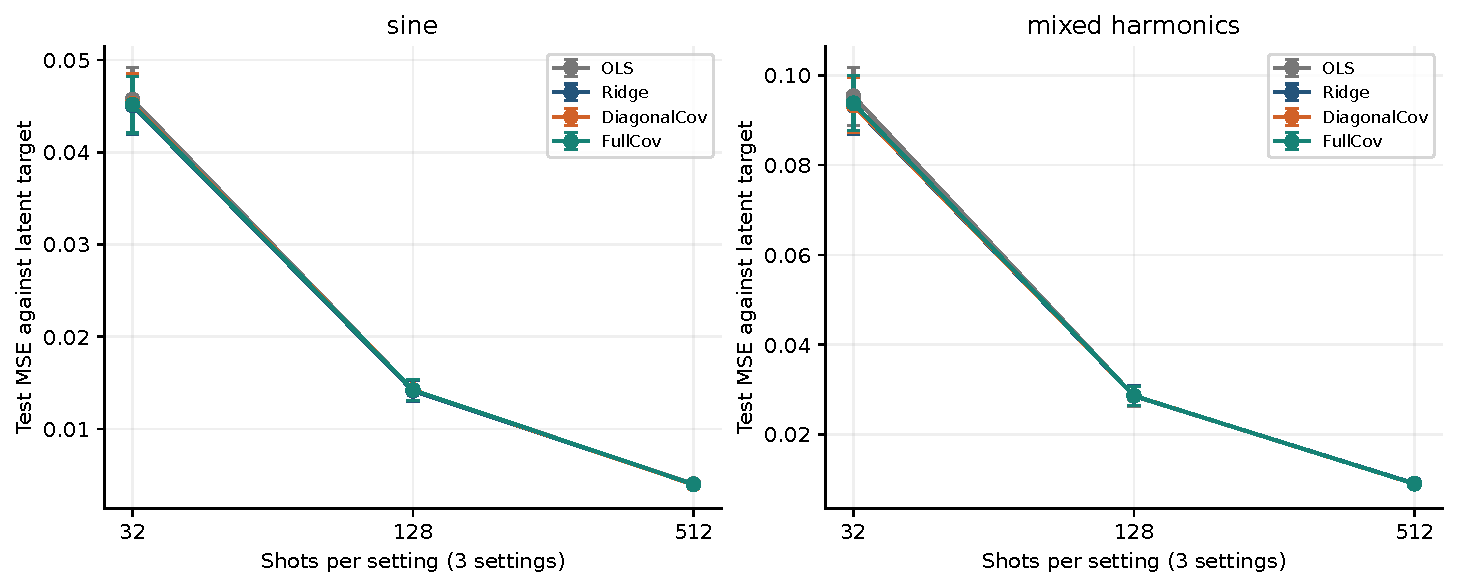
\includegraphics[width=0.94\textwidth]{extension_mse.pdf}
\caption{Fresh clean-label test MSE for four methods. The curves nearly overlap; error bars show sample SD across dataset-level acquisition means.}
\label{fig:mse}
\end{figure*}

\subsection{Diagonal Ablation and Penalty Selection}
FullCov has lower primary mean MSE than DiagonalCov in \AblationWins{} of six finite-shot settings. Retaining off-diagonal noise terms therefore does not produce a consistent benefit in this setup. FullCov selects $\gamma=0$ in approximately \GammaZeroMin{}--\GammaZeroMax{}\% of individual primary dataset/acquisition fits, depending on task and shot budget. Such choices switch off the covariance penalty and are not evidence that covariance helped.





\subsection{Separate Noisy-Label Sensitivity}
With training/validation label-noise SD 0.1, FullCov improves the finite-shot mean relative to Ridge in \NoisyWins{} of six settings, with small and mixed differences. Test targets remain noiseless. Exact-reference differences are unrelated to covariance because its value is zero. This sensitivity analysis does not reverse the primary conclusion.

\section{Verification and Reproducibility}
The combined suite has 54 passing automated tests. Covariance checks compare the weighted-count formula with explicitly expanded shot records, verify its expectation against a known distribution, and test symmetry, positive semidefiniteness, block structure and scaling. Further tests check the unpenalized intercept, gamma-zero Ridge equivalence, diagonal/full equality for diagonal noise, training-only preprocessing, invalid configuration rejection and full alternate-configuration execution.

An independent audit reconstructs all 300 training covariance estimates from expanded shots and refits all 124,160 candidates using augmented least squares rather than the production normal-equation solver. It checks all 5,120 saved readouts, coefficients, intercepts, scalers and prediction vectors, along with 64 summary groups and 64 paired contrasts. A separately expressed PennyLane circuit checks the probabilities at all 4,480 extension inputs. The original study also continues to pass its audit unchanged.

A fresh local run reproduces all extension metrics and fitted arrays; Linux verification also passes within stated floating-point tolerances. Integer counts and saved-file checksums remain exact. Passing checks does not exclude every possible scientific or implementation limitation.

The recorded environment uses Python 3.12.14, NumPy 2.3.5, SciPy 1.16.3, scikit-learn 1.7.2 and PennyLane 0.43.1. All experiments run on a CPU; a GPU or quantum processor is unnecessary for this simulation.

Raw measurements, fitted arrays, source snapshots and verification records are preserved in the project repository~\cite{repo}.

\section{Discussion and Limitations}
The experiment supports a limited conclusion: measurement-aware covariance penalties do not reliably improve this fixed two-qubit readout beyond the selected Ridge baseline. It does not show that such methods are ineffective generally, nor contradict results from different forecasting or trainable-circuit settings.

Possible limitations include estimation error in the penalty, only 32 validation inputs, the extra gamma-selection dimension and a competitive baseline. These are hypotheses rather than experimentally isolated causes of each failure. The diagonal/full comparison itself is mixed, which limits claims about the benefit of measured correlations.

The study uses two synthetic one-dimensional targets, one circuit, one split size and twenty independent dataset realizations in the extension. It includes no device errors, learned circuit, adaptive shot allocation or physical processor. No matched comparison of classical and quantum feature families is performed, so quantum advantage is not evaluated. The exact-feature reference remains diagnostic rather than a hardware procedure. The original study's full-rank local-feature matrices and the absence of an outcome-dimension sweep also prevent claims to reproduce the cited interpolation mechanisms.

Future work could evaluate alternative feature maps, more robust validation or a carefully matched reproduction of one reference. Designs chosen after examining these results require a new held-out evaluation. Covariance shrinkage or eigentask controls would be separately implemented and verified, not claimed as completed here.

\section{Conclusion}
This semester project implements a reproducible quantum-feature regression pipeline, extends it with training-measurement covariance penalties, and compares four readouts on fresh data under matched shot budgets. More shots improve average prediction performance in the tested settings. Full covariance regularization improves only one of six primary task/budget means and does not consistently beat its diagonal ablation. The contribution is a verified implementation and controlled assessment with preserved failure cases, not a new algorithm or guaranteed accuracy improvement.

\begin{thebibliography}{00}
\bibitem{kreplin} D. A. Kreplin and M. Roth, ``Reduction of finite sampling noise in quantum neural networks,'' \textit{Quantum}, vol. 8, Art. no. 1385, 2024, doi: 10.22331/q-2024-06-25-1385.
\bibitem{hu2023} F. Hu et al., ``Tackling sampling noise in physical systems for machine learning applications: Fundamental limits and eigentasks,'' \textit{Phys. Rev. X}, vol. 13, Art. no. 041020, 2023, doi: 10.1103/PhysRevX.13.041020.
\bibitem{baumann} M. Baumann, M. Zorn, T. Gabor, C. Linnhoff-Popien, and J. Stein, ``From quantum shots to training data: Reorganizing measurement records in quantum machine learning,'' arXiv:2604.28160v2, 2026, preprint. [Online]. Available: \url{https://arxiv.org/abs/2604.28160}
\bibitem{hu2024} F. Hu and X. Gao, ``Generalization error in quantum machine learning in the presence of sampling noise,'' arXiv:2410.14654, 2024, preprint. [Online]. Available: \url{https://arxiv.org/abs/2410.14654}
\bibitem{shots} G. Lo Monaco et al., ``Who can sample forever? Shot noise effects in quantum linear regression,'' arXiv:2610.12015, 2026, preprint. [Online]. Available: \url{https://arxiv.org/abs/2610.12015}
\bibitem{triple} G. Lo Monaco et al., ``Triple descent in quantum linear regression,'' arXiv:2611.00272, 2026, preprint. [Online]. Available: \url{https://arxiv.org/abs/2611.00272}
\bibitem{sklearn} Scikit-learn developers, ``Ridge,'' software documentation, accessed Nov. 23, 2026. [Online]. Available: \url{https://scikit-learn.org/stable/modules/generated/sklearn.linear_model.Ridge.html}
\bibitem{pennylane} PennyLane developers, ``Default qubit,'' software documentation, accessed Nov. 23, 2026. [Online]. Available: \url{https://docs.pennylane.ai/en/stable/code/api/pennylane.devices.default_qubit.html}
\bibitem{repo} K. Mehra, ``Quantum: Finite-shot quantum feature regression,'' project repository, 2026. [Online]. Available: \url{https://github.com/KartikMehra22/Quantum}
\end{thebibliography}
\end{document}
